\documentclass[%
 sor,
 jor,
 amsmath,amssymb,
 reprint,
]{revtex4-2}

\usepackage{graphicx}
\usepackage{xcolor}
\usepackage{siunitx}
\usepackage{dcolumn}
\usepackage{bm}
\usepackage{amsmath, amssymb, amsfonts}
\usepackage{placeins}
\usepackage{float}
\usepackage{pgfplots}
\pgfplotsset{compat=1.17}


\begin{document}

\title{Experiment 7\\Lee's Method}

\author{Aumshree P. Shah\\20231059}
\altaffiliation{\color{red}aumshree.pinkalbenshah@students.iiserpune.ac.in}
\date{\today}

\begin{abstract}
\centering
In this experiment the thermal conductivity of a bad conductor is measured.
\end{abstract}

\maketitle

\section{Theory and Procedure}
\subsection{Apparatus}
\small
\begin{minipage}{0.48\textwidth}
\begin{itemize}
	\item Lee’s Apparatus
	\item Bad conductor discs 
	\item Two thermometers
	\item Boiler and Induction
\end{itemize}
\end{minipage}
\begin{minipage}{0.48\textwidth}
\begin{itemize}
	\item Stop watch 
	\item Weighing balance 
	\item  Vernier Caliper 
	\item  Screw gauge
\end{itemize}
\end{minipage}
\subsection{Theory}
Fourier’s Law of heat conductance gives the rate of transfer of heat between two objects at temperatures T2 and T1 connected by a conductor with conductivity k and cross-sectional areas A (assumed uniform) and length l as %∆Q ∆t = k A l (T2 −T1) This equation governs the rate of heat transfer from disc D2 to D1 in the first half of the experiment. The instantaneous rate at which a warm body loses heat to surroundings is given by Newton’s law of cooling (which is a special case of Stefan’s law, when the temperature differences are small, and there are losses other than radiative losses). dT dt = −b(T −Ta), where Ta is the ambient temperature. This law governs the rate at which the disc D1 cools in the second half of the experiment. If m is the mass of the disk and s is the specific heat of the material of D1 (brass in this case), then the rate at which heat is lost by the disc D1 ∆Q1 ∆t = ms(dT1/dt) 


\subsection{Procedure}
\begin{enumerate}
\item Fill the boiler with water to nearly half and heat it to produce steam. In the mean time, weigh the disc D1 on which the apparatus rests. Further, measure the diameter of specimen disc d with a vernier calliper and its thickness using a screw gauge at several spaces and determine the mean thickness. Clamp the glass specimen between the base disk D2 of the steam jacket and the auxiliary brass disc D1. Insert the thermometers (either mercury thermometer or thermocouples) in the two brass disks D1,D2. Check if they show the same readings at room temperatu%re. If not, note the difference T ′. Connect the boiler outlet with the inlet of the steam chamber by a rubber tube. Continue passing steam until the two brass disks reach a steady temperature. Note down the temperatures T1 and T2 of the two discs. The second part of the experiment involves the determination of the cooling rate of disc D1 alone. Remove the sample disc. Heat the disc D1 directly by the steam chamber till its temperature is about T1 +1%0◦C. Remove the steam chamber and place the insulating disk on it. Record the temperature of the brass disc at half minute intervals. Continue till the temperature falls to about T1 −7◦

\end{enumerate}
\subsubsection{Precautions}
\begin{itemize}
\item PRECAUTIONS
\end{itemize}
\section{Observations}

\begin{table}[h]
\centering

Mass of D1 = % ADD A UNDERLINE HERE
in all variables add a underline



\begin{tabular}{|c|ccc|}
    \hline
    Material & $T_i$ (\si{\celsius})  & Length (cm) & $\Delta L$ ($10^{-5}$ m)\\
    \hline
    Copper 	& 24.0     & 59.8 & 75 \\
    Copper 	& 25.5-24.5-25.5 & 59.7 & 74\\
    Aluminium 	& 24.0-23.0-24.7 & 59.9 & 105\\
    Brass 	& 24.1-23.2-24.3 & 59.7 & 85 \\
    Steel 	& 22.1-24.8-20.5 & - & 74 \\
    Aluminium 	& 24.3-23.7-24.3 & 59.8 & 104\\
    Brass 	& 23.7-22.4-24.3 & 60.0 & 85 \\
    Steel 	& 24.6-25.3 & 59.9 & 76 \\
    Brass	& 24.8-25.3 & 60.1 & 86 \\
    Steel 	& 23.3-23.5 & 59.7 & 76 \\ 
    \hline
\end{tabular}
\caption{Data taken on 11 Mar 2025, the variables represents the property as described in the theory.}
\end{table}
Least count of scale: 0.1 cm  \\
Least count of thermometer: 0.1 $\si{\celsius}$ \\
Least count of spherometer: $10^{-5}$ m  \\


\section{Uncertainties and Error Sources}
\subsection{Measurement Uncertainties}
\begin{itemize}
    \item \textbf{Length Measurements:} Estimated uncertainty of $\pm 0.1$ cm due to not proper method of viewing, expansion uncertainty of $\pm 5\times 10^{-6}$ m.
    \item \textbf{Temperature Measurements:} Uncertainty of $\pm 0.05$ \si{\kelvin} due to instrument resolution.
\end{itemize}

\subsection{Random Errors}
\begin{itemize}
	\item Errors in the final value of $\alpha$ due to different rods having different material composition 
\end{itemize}
\subsection{Systematic Errors}
\begin{itemize}
	\item Errors from the uneven temperature of the rod during the initial temperature measurement
	\item Improper contact between the thermometer and the metal rod during temperature measurement
\end{itemize}



\section{Calculation and Error Analysis}
\subsection{Error Propagation}
From the length and temperature uncertanity, the formula given in the thory the uncertanity will travel as: REFRENCE THE BOOOkThe uncertainty in $\alpha$ is given by the basic formula for error propagation.:
\[
\sigma_{\alpha} = \alpha \sqrt{\left( \frac{\sigma_{\Delta L}}{\Delta L} \right)^2 + \left( \frac{\sigma_L}{L} \right)^2 + \left( \frac{\sigma_{\Delta T}}{\Delta T} \right)^2}
\]
where $\sigma_{\Delta L}, \sigma_L, \sigma_{\Delta T}$ are the uncertainties in expansion length, initial length, and temperature difference, respectively.

\subsection{Calculation}
We calculate the value of $\alpha$ of all data points and their uncertainity from hte above formul,  we get:\footnote{Refer to \cite{github} for calculations}

\begin{table}[h]
\centering
\begin{tabular}{ccc}
\hline
Material & $\alpha$ (\si{1/\degreeCelsius}) \\
\hline
Aluminium & $(2.303 \pm 0.005) \times 10^{-5}$ \\
Aluminium & $(2.291\pm 0.005) \times 10^{-5}$ \\
Brass & $(1.870\pm 0.004) \times 10^{-5}$ \\
Brass & $(1.851\pm 0.004) \times 10^{-5}$ \\
Brass & $(1.909\pm 0.004) \times 10^{-5}$ \\
Copper & $(1.650\pm 0.003) \times 10^{-5}$ \\
Copper & $(1.656\pm 0.003) \times 10^{-5}$ \\
Steel & $(1.591\pm 0.003) \times 10^{-5}$ \\
Steel & $(1.691\pm 0.003) \times 10^{-5}$ \\
Steel & $(1.662\pm 0.003) \times 10^{-5}$ \\
\hline


\end{tabular}
\caption{Calculated expansion coefficients}
\end{table}

\section{Result}
The calculated values of $\alpha$ show high precision but large variations from expected values. The inconsistencies suggest experimental errors, leading to unreliable results.

















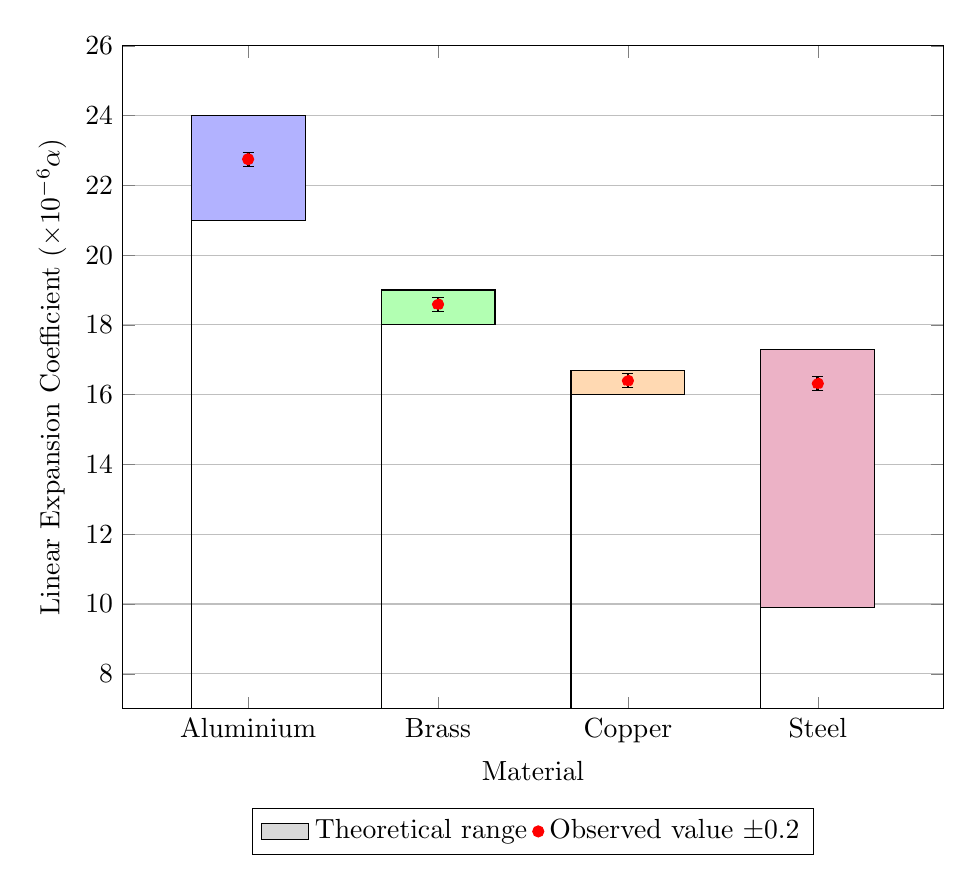
\begin{tikzpicture}
  % Set up the axis with custom dimensions, white background,
  % and y-axis starting at 7 for better visibility of error bars.
  \begin{axis}[
      width=12cm,
      height=10cm,              % Increased height for clear error bar visibility
      xlabel={Material},
      ylabel={Linear Expansion Coefficient ($\times 10^{-6} \alpha$)},
      xtick={1,2,3,4},
      xticklabels={Aluminium, Brass, Copper, Steel},
      ymin=7, ymax=26,          % y-axis range from 7 to 26
      ymajorgrids=true,
      axis background/.style={fill=white}, % Set the background to white instead of pink
      legend style={at={(0.5,-0.15)},anchor=north,legend columns=2},
  ]

  % Add legend entries:
  % - Theoretical range (displayed as a colored rectangle)
  % - Observed value with error bars (red dot with black error bars)
  \addlegendimage{area legend, fill=gray!30, draw=black}
  \addlegendentry{Theoretical range}
  \addlegendimage{only marks, mark=*, mark options={red}}
  \addlegendentry{Observed value $\pm0.2$}

  %-------------------------------
  % Plot theoretical ranges as colored rectangles
  % Each rectangle represents the range for the material.
  % The width of 0.6 units (from x-0.3 to x+0.3) centers the rectangle at the xtick.
  
  % Aluminium: theoretical range [21, 24]
  \addplot [draw=black, fill=blue!30] coordinates {
    (1-0.3,21) % Bottom left corner
    (1+0.3,21) % Bottom right corner
    (1+0.3,24) % Top right corner
    (1-0.3,24) % Top left corner
  } \closedcycle; % Close the cycle to form a rectangle

  % Brass: theoretical range [18, 19]
  \addplot [draw=black, fill=green!30] coordinates {
    (2-0.3,18)
    (2+0.3,18)
    (2+0.3,19)
    (2-0.3,19)
  } \closedcycle;

  % Copper: theoretical range [16, 16.7]
  \addplot [draw=black, fill=orange!30] coordinates {
    (3-0.3,16)
    (3+0.3,16)
    (3+0.3,16.7)
    (3-0.3,16.7)
  } \closedcycle;

  % Steel: theoretical range [9.9, 17.3]
  \addplot [draw=black, fill=purple!30] coordinates {
    (4-0.3,9.9)
    (4+0.3,9.9)
    (4+0.3,17.3)
    (4-0.3,17.3)
  } \closedcycle;

  %-------------------------------
  % Plot observed values with error bars:
  % The observed values are marked with red dots.
  % The error bars are drawn with a solid, dark black line and the caps are filled black.
  % The error bars extend ±0.2 in the y-direction.
  \addplot+[
      only marks,
      mark=*,
      mark options={red}, % Red dot for the observed value
      error bars/.cd,
      y dir=both,        % Error bars in both upward and downward directions
      y explicit,        % Use the explicit error value provided
      error bar style={color=black, line width=1pt, solid}, % Solid, dark black error bars
 %     error mark options={draw=black, fill=black, solid} % Filled black error bar caps
  ] coordinates {
      (1,22.75) +- (0,0.2) % Aluminium observed value with ±0.2 error
  };

  \addplot+[
      only marks,
      mark=*,
      mark options={red},
      error bars/.cd,
      y dir=both,
      y explicit,
      error bar style={color=black, line width=1pt, solid},
  ] coordinates {
      (2,18.59) +- (0,0.2) % Brass observed value with ±0.2 error
  };

  \addplot+[
      only marks,
      mark=*,
      mark options={red},
      error bars/.cd,
      y dir=both,
      y explicit,
      error bar style={color=black, line width=1pt, solid},
  ] coordinates {
      (3,16.4) +- (0,0.2) % Copper observed value with ±0.2 error
  };

  \addplot+[
      only marks,
      mark=*,
      mark options={red},
      error bars/.cd,
      y dir=both,
      y explicit,
      error bar style={color=black, line width=1pt, solid},
  ] coordinates {
      (4,16.32) +- (0,0.2) % Steel observed value with ±0.2 error
  };

  \end{axis}
\end{tikzpicture}






















% CHANGE THEO: https://en.wikipedia.org/wiki/Thermal_expansion


\vspace{1cm}

\noindent\fbox{%
    \parbox{\textwidth}{%
    Lets fucking go   

    }%
}\\

\noindent\rule{\linewidth}{0.4pt}
\hfill

\appendix
\section{Theoretical Values}
The expected values of $\alpha$ in \si{\per\celsius} are:\footnote{\cite{alpha}}
\[
\begin{split}
\alpha_{\text{Steel}} &\approx (1.08 - 1.25) \times 10^{-5}\\
\alpha_{\text{Brass}} &\approx (1.8 - 1.9) \times 10^{-5}\\
\alpha_{\text{Aluminium}} &\approx (2.1 - 2.4) \times 10^{-5}\\
\alpha_{\text{Copper}} &\approx 1.78 \times 10^{-5}
\end{split}
\]

\bibliography{aipsamp}
\end{document}
